% Pins & connections reference for the Parkinson's closed-loop gait garment.
% ENGF0031 Scenario 2.  Build with tectonic (XeLaTeX):  tectonic wiring_pinout.tex
% Architecture: CPX (sense + cue) --UART--> ESP32 (Wi-Fi bridge) --TCP--> laptop (CNN).
\documentclass[11pt]{article}

\usepackage[a4paper,margin=2cm]{geometry}
\usepackage[table]{xcolor}
\usepackage{booktabs}
\usepackage{array}
\usepackage{tabularx}
\usepackage{enumitem}
\usepackage{titlesec}
\usepackage{tikz}
\usepackage{circuitikz}
\usetikzlibrary{arrows.meta,positioning}

% ── palette (matches the coding flowchart: slate line-work, terracotta accent) ──
\definecolor{slate}{HTML}{3D4A57}
\definecolor{accent}{HTML}{8F3322}
\definecolor{slatebg}{HTML}{EEF1F4}
\definecolor{rule}{HTML}{C2CCD4}

\titleformat{\section}{\large\bfseries\color{slate}}{}{0pt}{}
\titlespacing*{\section}{0pt}{12pt}{5pt}

% wrapping table columns
\newcolumntype{L}{>{\raggedright\arraybackslash}X}
\newcommand{\hdr}[1]{{\color{white}\textbf{#1}}}
\setlist[itemize]{leftmargin=1.4em,itemsep=1pt,topsep=2pt}

\pagestyle{empty}

\begin{document}

% ── title block ──
\begin{center}
  {\LARGE\bfseries Pins \& Connections}\\[3pt]
  {\large Parkinson's Closed-Loop Gait Garment \textemdash{} ENGF0031 Scenario 2}\\[3pt]
  {\color{slate}\small Circuit Playground Express \quad+\quad ESP32 (Wi-Fi bridge) \quad+\quad laptop (wireless)}
\end{center}
\vspace{2pt}
{\color{rule}\hrule height 1pt}
\vspace{8pt}

\noindent
The wearable is now \textbf{untethered}. The Circuit Playground Express (CPX) does all the
sensing and drives the cue; a small \textbf{ESP32} relays data to and from the laptop
over \textbf{Wi-Fi}; and the laptop runs the CNN that makes the freeze decision. CPX and ESP32 talk
over a short \textbf{UART} link \textemdash{} both are 3.3\,V logic, so they connect directly with
\emph{no level shifter}. The motor-driver wiring is unchanged from the earlier builds; only the
\emph{link to the laptop} has changed (a Wi-Fi hop via the ESP32 instead of a USB cable).

% ════════════════════════════════════════════════════════════════════
\section{System overview --- where the data goes}
\begin{center}
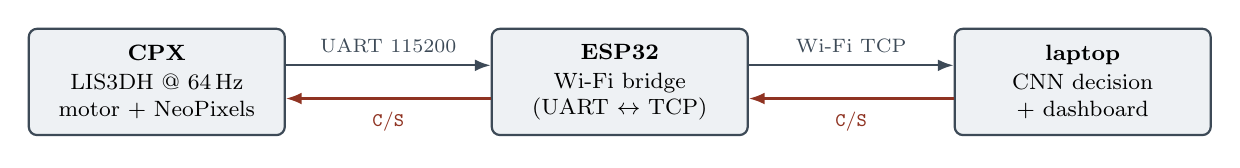
\begin{tikzpicture}[
   font=\footnotesize,
   box/.style={draw=slate, line width=0.8pt, rounded corners=3pt, fill=slatebg,
               align=center, inner sep=5pt, minimum height=1.35cm, text width=2.9cm},
   fwd/.style={-{Latex[length=2mm]}, line width=0.8pt, color=slate},
   cue/.style={-{Latex[length=2mm]}, line width=0.8pt, color=accent},
]
  \node[box] (cpx) {\textbf{CPX}\\[1pt] LIS3DH @ 64\,Hz\\ motor + NeoPixels};
  \node[box, right=2.6cm of cpx] (esp) {\textbf{ESP32}\\[1pt] Wi-Fi bridge\\ (UART $\leftrightarrow$ TCP)};
  \node[box, right=2.6cm of esp] (pi)  {\textbf{laptop}\\[1pt] CNN decision\\ + dashboard};
  \draw[fwd] ([yshift=6pt]cpx.east) -- ([yshift=6pt]esp.west)
        node[midway, above=1pt, font=\scriptsize, color=slate]{UART 115200};
  \draw[cue] ([yshift=-6pt]esp.west) -- ([yshift=-6pt]cpx.east)
        node[midway, below=1pt, font=\scriptsize, color=accent]{\texttt{C}/\texttt{S}};
  \draw[fwd] ([yshift=6pt]esp.east) -- ([yshift=6pt]pi.west)
        node[midway, above=1pt, font=\scriptsize, color=slate]{Wi-Fi TCP};
  \draw[cue] ([yshift=-6pt]pi.west) -- ([yshift=-6pt]esp.east)
        node[midway, below=1pt, font=\scriptsize, color=accent]{\texttt{C}/\texttt{S}};
\end{tikzpicture}\\[3pt]
{\footnotesize\color{slate} Accelerometer stream flows right (\texttt{ax,ay,az} at 64\,Hz); the freeze-cue command (\texttt{C}/\texttt{S}) returns left.}
\end{center}

% ════════════════════════════════════════════════════════════════════
\section{Board pin map --- Circuit Playground Express}

\renewcommand{\arraystretch}{1.25}
\begin{tabularx}{\textwidth}{l l l L}
  \toprule
  \rowcolor{slate}
  \hdr{Pin / pad} & \hdr{Direction} & \hdr{Connects to} & \multicolumn{1}{l}{\hdr{Purpose}} \\
  \midrule
  \texttt{A1}   & digital out   & $1\,\mathrm{k}\Omega \rightarrow$ Q1 base & switches the vibration motor (the cue) \\
  \texttt{A7}   & UART TX (out) & ESP32 \texttt{GPIO16} (RX2)               & \texttt{Serial1} TX --- streams \texttt{ax,ay,az} to the ESP32 \\
  \texttt{A6}   & UART RX (in)  & ESP32 \texttt{GPIO17} (TX2)               & \texttt{Serial1} RX --- receives the \texttt{C}/\texttt{S} cue \\
  \texttt{VOUT} & power (3.3\,V)& motor\,(+), diode cathode                 & board-regulated rail; supplies the motor \\
  \texttt{GND}  & power (0\,V)  & Q1 emitter, motor return                  & common ground --- shared with the ESP32 \\
  \texttt{A0}   & ---           & left open (unused)                        & onboard speaker/DAC pin --- \textbf{avoid} \\
  micro-USB     & 5\,V in       & USB power bank / charger                  & \textbf{power only} now; optional debug serial \\
  Button A      & onboard input & ---                                       & hold still + press to calibrate the energy floor \\
  Slide switch  & onboard input & ---                                       & cue master-enable (wearer can silence it) \\
  NeoPixels $\times$10 & onboard output & ---                               & state indicator (see legend below) \\
  LIS3DH accel  & onboard (I\textsuperscript{2}C) & ---                     & 3-axis accelerometer, sampled at 64\,Hz \\
  \bottomrule
\end{tabularx}

% ════════════════════════════════════════════════════════════════════
\section{CPX $\leftrightarrow$ ESP32 --- the UART link}

\noindent
Three wires carry exactly the bytes the old USB cable used to. \texttt{TX} and \texttt{RX}
\textbf{cross over}, and the two boards \textbf{must share a ground}. Both run at 3.3\,V, so the
lines connect directly --- no level shifter, no divider.

\vspace{4pt}
\renewcommand{\arraystretch}{1.25}
\begin{tabularx}{\textwidth}{l c l L}
  \toprule
  \rowcolor{slate}
  \hdr{CPX pad} & \hdr{} & \hdr{ESP32 pin} & \multicolumn{1}{l}{\hdr{Signal}} \\
  \midrule
  \texttt{A7} (TX / D1) & $\rightarrow$ & \texttt{GPIO16} (RX2) & accel stream \texttt{ax,ay,az}, 64\,Hz \\
  \texttt{A6} (RX / D0) & $\leftarrow$  & \texttt{GPIO17} (TX2) & cue command \texttt{C} / \texttt{S} \\
  \texttt{GND}          & ---           & \texttt{GND}          & common ground --- \textbf{mandatory} \\
  \bottomrule
\end{tabularx}

\vspace{3pt}
{\footnotesize\noindent\textbf{\color{slate}Notes.}\;
115200\,baud, 8N1 (same framing as the old USB link).
\texttt{GPIO16}/\texttt{17} are the ESP32's default \texttt{Serial2} pins on a WROOM DevKitC; on
WROVER modules those pins are used by the PSRAM, so pick two free GPIOs (e.g.\ \texttt{25}/\texttt{26})
and pass them to \texttt{Serial2.begin()}. Keep the wires short and do \emph{not} also link the two
3.3\,V rails --- power each board on its own.\par}

% ════════════════════════════════════════════════════════════════════
\section{Motor driver --- off-board components}

\noindent
\begin{minipage}[t]{0.46\textwidth}
  \vspace{2pt}
  A CPX pad can only source a few mA, but the coin motor draws $\sim$90\,mA, so pad
  \texttt{A1} \emph{switches} a transistor that passes the motor current from \texttt{VOUT}:
  \begin{itemize}
    \item \texttt{A1} $\rightarrow$ R1 ($1\,\mathrm{k}\Omega$) $\rightarrow$ Q1 \textbf{base}
    \item Q1 \textbf{emitter} $\rightarrow$ \texttt{GND}
    \item Q1 \textbf{collector} $\rightarrow$ motor\,($-$)
    \item motor\,($+$) $\rightarrow$ \texttt{VOUT} (3.3\,V)
    \item D1 across the motor, \textbf{cathode} $\rightarrow$ motor\,($+$)/\texttt{VOUT}
  \end{itemize}
\end{minipage}\hfill
\begin{minipage}[t]{0.50\textwidth}
  \centering
  \vspace{-2pt}
  \begin{circuitikz}[american, scale=0.92, transform shape]
    \node[npn, anchor=B](Q) at (0,0){};
    % base resistor from the A1 pad
    \draw (Q.B) to[R, l=$1\,\mathrm{k}\Omega$, -*] ++(-3.0,0)
          node[left, align=right, font=\footnotesize]{pad \texttt{A1}};
    % emitter to ground
    \draw (Q.E) -- ++(0,-1.0) node[ground]{};
    % collector up to motor(-)
    \draw (Q.C) -- ++(0,0.7) coordinate(mn);
    % motor up to VOUT(+)
    \draw (mn) to[generic, l=motor] ++(0,2.0) coordinate(vt);
    \draw (vt) -- ++(0,0.5) node[above, font=\footnotesize]{\texttt{VOUT} 3.3\,V};
    \node[left, font=\footnotesize] at (vt) {$+$};
    \node[left, font=\footnotesize] at (mn) {$-$};
    % flyback diode in parallel, cathode at top (VOUT side)
    \draw (mn) -- ++(1.7,0) coordinate(d0);
    \draw (d0) to[D, l_={1N4148}] ++(0,2.0) coordinate(d1);
    \draw (d1) -- (vt);
    % transistor label
    \node[font=\footnotesize, anchor=west] at (1.15,-0.15){Q1};
  \end{circuitikz}\\[2pt]
  {\footnotesize\color{slate} low-side NPN switch}
\end{minipage}

\vspace{8pt}
\renewcommand{\arraystretch}{1.2}
\begin{tabularx}{\textwidth}{l l l L}
  \toprule
  \rowcolor{slate}
  \hdr{Ref} & \hdr{Part} & \hdr{Value / type} & \multicolumn{1}{l}{\hdr{Function}} \\
  \midrule
  Q1 & NPN BJT              & 2N2222 / BC547      & low-side switch driven by \texttt{A1} \\
  R1 & resistor             & $1\,\mathrm{k}\Omega$ & limits base current from the 3.3\,V pad \\
  D1 & diode                & 1N4148              & flyback --- clamps the motor's inductive spike at switch-off \\
  M1 & coin vibration motor & $\sim$3\,V, $\sim$90\,mA & the rhythmic vibrotactile gait cue \\
  \bottomrule
\end{tabularx}

% ════════════════════════════════════════════════════════════════════
\section{ESP32 connections}

\renewcommand{\arraystretch}{1.25}
\begin{tabularx}{\textwidth}{l l l L}
  \toprule
  \rowcolor{slate}
  \hdr{ESP32 pin} & \hdr{Direction} & \hdr{Connects to} & \multicolumn{1}{l}{\hdr{Purpose}} \\
  \midrule
  \texttt{GPIO16} (RX2) & UART in     & CPX \texttt{A7} (TX)            & receives the accel stream from the CPX \\
  \texttt{GPIO17} (TX2) & UART out    & CPX \texttt{A6} (RX)            & sends the \texttt{C}/\texttt{S} cue to the CPX \\
  \texttt{GND}          & power (0\,V)& CPX \texttt{GND}, battery ($-$) & common ground \\
  \texttt{5V} / \texttt{VIN} & power in & USB power bank / battery ($+$) & board supply (on-board 3.3\,V regulator) \\
  Wi-Fi radio           & ---         & laptop network                   & TCP socket to the laptop, $\sim$64\,Hz \\
  \bottomrule
\end{tabularx}

% ════════════════════════════════════════════════════════════════════
\section{Host link --- Wi-Fi to the laptop}

\noindent
The ESP32 joins the same Wi-Fi network as the laptop (or the laptop's own hotspot) and opens a
\textbf{TCP socket} to it. It forwards every accelerometer line it gets from the CPX and relays
the laptop's cue commands back. The payloads are unchanged from the old USB link --- only the
transport differs, so everything downstream on the laptop (the CNN, the dashboard) is untouched: the
laptop simply reads a \textbf{socket} instead of \texttt{/dev/ttyACM0}.

\vspace{4pt}
\renewcommand{\arraystretch}{1.25}
\begin{tabularx}{\textwidth}{l l L}
  \toprule
  \rowcolor{slate}
  \hdr{Direction} & \hdr{Payload} & \multicolumn{1}{l}{\hdr{Rate / format}} \\
  \midrule
  CPX $\rightarrow$ ESP32 $\rightarrow$ laptop & \texttt{ax,ay,az} (newline-terminated) & 64\,Hz, three int16 in milli-g (CSV) \\
  laptop $\rightarrow$ ESP32 $\rightarrow$ CPX & \texttt{C} = start cue,\; \texttt{S} = stop cue & one character, sent on a state change \\
  \bottomrule
\end{tabularx}

\vspace{4pt}
\noindent
In the \emph{standalone} build the CPX computes the Freeze Index itself and drives the motor with
no ESP32 or laptop attached --- the wireless link is only for the CNN (full-PyTorch) build.

% ════════════════════════════════════════════════════════════════════
\section{NeoPixel state legend}

\noindent
\begin{tabular}{@{}ll@{}}
  \tikz\fill[green!55!black] (0,0) circle (3.4pt); & \textbf{Green} --- walking / monitoring \\[3pt]
  \tikz\fill[accent] (0,0) circle (3.4pt);          & \textbf{Red (pulsing)} --- actively cueing \\[3pt]
  \tikz\fill[teal!55!gray] (0,0) circle (3.4pt);    & \textbf{Dim teal} --- standing still (gate holding the cue off) \\[3pt]
  \tikz\fill[blue!70] (0,0) circle (3.4pt);         & \textbf{Blue} --- calibrating the still-floor \\
\end{tabular}

% ── caution box ──
\vspace{10pt}
\noindent\fcolorbox{accent}{accent!6}{%
  \begin{minipage}{\dimexpr\textwidth-2\fboxsep-2\fboxrule}
    \small\textbf{\color{accent}Power \& safety.} The wearable now runs on \textbf{battery}
    (a USB power bank or a LiPo) --- power the CPX and the ESP32 each from their own 5\,V input and
    \textbf{tie their grounds together}; do not cross-link the two 3.3\,V rails. The motor's
    $\sim$90\,mA is switched from \texttt{VOUT}; the \textbf{1N4148 flyback diode is mandatory} to
    protect Q1 from the inductive kick at switch-off. The laptop is self-powered (its own battery/charger) and shares no power rail with the wearable. \texttt{A0} is left unconnected (onboard speaker/DAC), and the UART link needs a
    \textbf{shared ground} and short wires to stay reliable.
  \end{minipage}}

\end{document}
